\documentclass{standalone}
\usepackage{currfile}
\usepackage{tikz}
\usepackage[mode=buildnew]{standalone}
\usetikzlibrary{spy}
\tikzset{
	mirror scope/.is family,
	mirror scope/angle/.store in=\mirrorangle,
	mirror scope/center/.store in=\mirrorcenter,
	mirror setup/.code={\tikzset{mirror scope/.cd,#1}},
	mirror scope/.style={mirror setup={#1},spy scope={
	rectangle,lens={rotate=\mirrorangle,yscale=-1,rotate=-1*\mirrorangle},size=80cm}},
}
\newcommand\mirror[1][]{\spy[overlay,#1] on (\mirrorcenter) in node at (\mirrorcenter)}

\begin{document}
	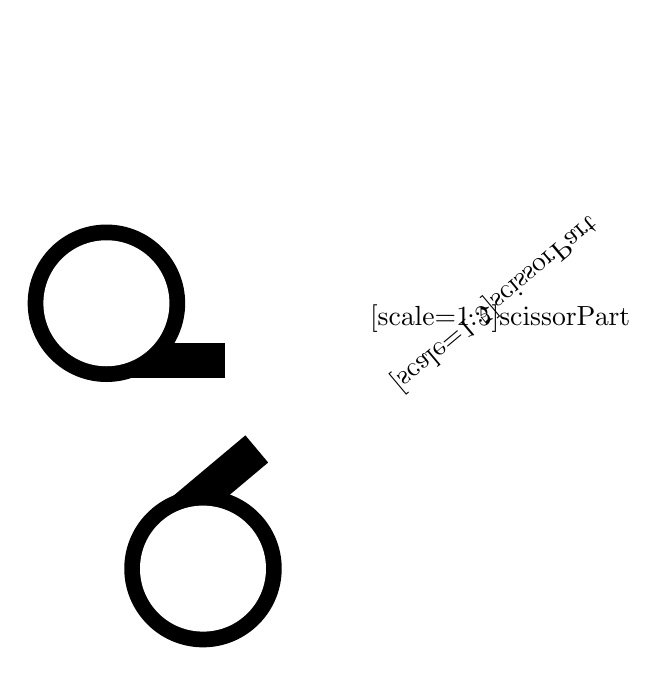
\begin{tikzpicture}
		\fill[white] (0,-4.5) rectangle (5,3.5);
%		\fill[black] (0,-0.5) rectangle (1.5,-0.95);
%		\node[draw=none,fill=none] at (5,-0.2) {\includestandalone[scale=1.5]{./scissorPart}};
%		\fill[black] (0,0) circle (1);
		\begin{scope}[mirror scope={center={-3,-3},angle=20},yshift=0cm]
			\fill[black] (0,-0.5) rectangle (1.5,-0.95);
			\node[draw=none,fill=none] at (5,-0.2) {\includestandalone[scale=1.5]{\currfiledir scissorPart}};
			\fill[black] (0,0) circle (1);
			\fill[white] (0,0) circle (0.8);
			\mirror;
		\end{scope}
	\end{tikzpicture}
\end{document}
